\documentclass[../report]{subfiles}
\setcounter{section}{0}
\begin{document}

本章では,システム開発の詳細について説明する.
\bunseki{佐藤碧}


\section{カメラの実装}
\subsection{利用した技術} \label{sec:used-camera-technology}
本システムでは,動体を自動で検出して画像を撮影し,それをサーバに送信できるようにする必要がある.
それらを実現するためには幾つかの方法が考えられるが,私たちはマイコンの一種であるRaspberry Piを用いることにした.
本システムでは,ボックスにカメラを取り付けて画像を撮影する.
その際,カメラを含めた機器類はなるべく小型であるほうが,カメラを取り付ける際の都合がよい.
例えば,取り付けた際のボックスの外観をシンプルにできるということが挙げられる.
それにより,取り付けた機器類が目立ちにくくでき,ユーザが不用意に触ってしまうことで不具合が起きる事態を防げる.
また,動体検出,画像撮影,画像の送信といった機能に必要となるリソースは,それほど膨大なわけではない.
よって,通常のコンピュータと比較すると小型である代わりに非力であるRaspberry Piを用いても,必要な機能を実現できると考えた.
以上のような理由から,私たちはRaspberry Piを用いることにした.

動体の自動検出と画像の撮影には,Raspberry PiのパッケージであるMotionを利用した.
MotionはRaspberry Piに接続されたカメラを通して動体を検出して画像を撮影することができるパッケージである.
Motoiinは一度動体を検出すると,動体の検出が終了するまでの間に連続して画像を撮影し続ける仕組みになっている.
また,パラメータを変更することによって動体検出の感度を調整することができる.
加えてMotionでは,動体検出で発生するイベントにフックさせて,任意のプログラムを実行させることが可能である.
発生するイベントの内,今回利用したのは以下の3種類である.
\begin{description}
    \item{onEventStart} 動体を検出し,画像を撮影しはじめたとき
    \item{onPictureSave} 動体検出中に画像を撮影して保存したとき
    \item{onEventEnd} 動体検出が終了したとき
\end{description}
\bunseki{佐藤碧}

\subsection{動体検出の問題点} \label{sec:problem-detect-motion}
\ref{sec:used-camera-technology}でも述べたように,Motionは動体検出ができる.
しかし,ここで一つの問題が浮上してくる.
それは,Motionの性質上,ボックス内に食事を置く際でも取り出す際でも,等しく動体検出を行い画像を撮影してしまうということである.
したがって,単純に動体検出が終了した際に最後に撮影した画像を送信するという処理を行うと,ボックス内に食事を置いた際はきちんと画像が撮影されてそれがサーバに送信されるが,ボックス内から食事を取り出した際にも同様に画像が撮影されサーバに送信されてしまう.
つまりは,本来不要な画像がサーバに送信されてしまうということである.
この問題に対しては,以下の2つの解決方法が考えられる.
\begin{enumerate}
    \item 画像が送信されるサーバ側で画像の選別を行い,必要とされる画像だけを利用するようにする方法
    \item 画像を送信する前にRaspberry Pi内で画像の選別を行い,必要となる画像だけをサーバに送信する方法
\end{enumerate}
今回は,後者の方法を取ることにした.
理由は,可能な限り,問題をそれが起きている範囲で解決できたほうが複雑にならなくて済むからである.
つまり,画像を送信する際に起きる問題は,画像を受信する側ではなく画像を送信する側で解決するべきであるということである.
このように,問題の発生箇所とそれを解決する箇所をなるべく近くにしておくことで,バグが発生した際に修正するべき箇所を発見しやすいという利点もある.

画像の選別は背景差分法を用いて行う.
背景差分法とは,物体が写っているか調べたい画像と事前に背景用として用意しておいた画像とをピクセル単位で比較し,相違点が多ければ物体が写っていると判断し,そうでなければ物体は写っていないと判断するといった手法である.
背景差分法はその性質上,固定カメラとの相性が良い.
なぜなら,固定カメラは背景画像に変化が生じにくいからである.
そのため,カメラに動体が写り込んだ際に検出がしやすいのである.
このような理由から,今回は背景差分法を用いることにした.

実装はPythonと画像処理ライブラリであるOpenCVを用いて行った.
実装した処理は以下のとおりである.
\begin{enumerate}
    \item 背景用に利用する画像を手動で撮影しておく
    \item 差分画像の2値化用とピクセル数用の閾値を設定しておく
    \item 食事の画像をサーバへ送信する際に判定を行う
    \begin{enumerate}
        \item 背景用の画像と送信する画像をグレースケールに変換する
        \item グレースケールに変換した背景用の画像と送信する画像について差分の絶対値を計算し,差分画像を取得する
        \item 事前に設定していた閾値を用いて差分画像を2値化する
        \item 2値化した差分画像の0でないピクセルの総数を求める
        \item 求めたピクセルの総数が閾値を上回っていれば画像を送信し,下回っていれば画像の送信をキャンセルする
    \end{enumerate}
\end{enumerate}
\bunseki{佐藤碧}

\subsection{背景差分法の精度における問題点}
\ref{sec:problem-detect-motion}にて,動体検出時における問題の解決を図った.
しかし残念ながら,精度はまだまだ不十分であった.
一定の効果は認められたものの,実際には本来送信するべきでない食事が写っていない画像を送信してしまうことがある.
したがって,サーバに食事が写っていない画像が送信されてしまうといった問題は完全に解決できたとはいえない.
その原因としては,ボックス内に写り込んでしまう影の影響が考えられる.
今回実装したアルゴリズムでは,動体検出のパラメータに画像の輝度のみを用いている.
しかし,影が映り込むことによって画像の輝度が容易に変化してしまうのである.
したがって,食事が写っていない画像に影が写り込んでしまった場合,画像の輝度が変化してしまうことにより,背景用の画像との差分が大きくなってしまう.
それにより,本来であれば背景用の画像との差分が小さいと判断され,サーバへの送信をキャンセルされるべき画像が,誤って送信されてしまうのである.

今回,背景差分法を用いるために実装したプログラムで利用しているアルゴリズムは,とても単純なものであった.
そして,単純なアルゴリズムは単純な動作しかできないため,複雑な条件が様々に絡み合う現実の問題に対しては対処しきれない.
背景差分法においてもそれは同様である.
今回のアルゴリズムの問題点は,画像同士の輝度の差という単純且つ単一のパラメータのみを利用していることにある.
この問題を解決するためには,例えば以下のような方法が考えられる.
\begin{enumerate}
    \item \label{enum:rgb-hsb} RGBやHSBといった多次元の値をもつ要素を比較のパラメータに用いた方法
    \item \label{enum:brightness-diff} 画像全体の輝度を利用した相対的な比較手法を用いる方法
    \item \label{enum:machine-learning} 機械学習を用いた画像認識による方法
\end{enumerate}
\ref{enum:rgb-hsb}の方法は,影の影響を受けやすい輝度を利用した比較ではなく,画像のRGBデータを正規化した色度や色相・彩度・明度の3要素からなるHSBと利用するという方法である.
\ref{enum:brightness-diff}の方法は,画像の輝度を正規化することで,画像を輝度を要素とした大きさが1のベクトルとして捉えることが可能になり,それを用いることで影による画像の輝度の変化を無視するという方法である.
\ref{enum:machine-learning}の方法は,認識させたい物体の特徴をコンピュータに学習させることで,画像にどのようなものが写っているかを自動で判別させるという方法である.
上記のような方法を用いることで,少なくとも現状よりは問題を改善できると考えられる.
\bunseki{佐藤碧}


\section{Webサーバの実装}
Webサーバのソースコード管理にはGit及びGitHubを使用した.
また,Gitフローを導入し,developブランチで後述のHerokuサーバにデプロイされるようにした.

Webサーバの実装には,RubyのWebフレームワークであるRuby on Railsを使用した.
Webフレームワークの使用に至った経緯は,3.2.2にて述べる.
ユーザには1人1アカウントが割り当てられ,それぞれ閲覧できる・閲覧されるユーザが指定できるよう多対多のリレーションを構築した.

ユーザが箱を通して送る毎日の食事の画像は,当初はGoogle Cloud Storageに保存する予定であったが,使用したライブラリでは正常にアップロードすることができなかったため,保存先をAmazon S3に変更した.
また,食事の画像が保存されると同時にジョブがキュー上に登録され,順に料理画像認識が実行される.
ジョブの管理には,一般のWebサービスで広く使われているライブラリであるsidekiqを使用している.
ジョブはRedis上に保存され,順次実行される.
この画像認識は別のAPIサーバ上で実行され,その実装については6.3にて述べる.
APIサーバから画像認識の結果が返ってくると,食事と料理の紐付けが保存される.

料理とその料理の一般的な栄養価の対応表は,あらかじめデータベースに用意しておき,画像認識で返ってくる料理名と一致することで,カメラに写った食事の栄養価が分かるというような実装とした.
また用意したデータベースに認識結果の料理名のものが入っていない場合は,ユーザがWebブラウザを介して登録できるようにした.

Webブラウザから見る画面やテレビの画面に表示する,一日の栄養摂取基準と比較してどのくらいの栄養を摂取しているかを示すレーダーチャートを実装している.
これもあらかじめ厚生労働省が公表している一日の栄養摂取基準から,カロリー・タンパク質・脂質・炭水化物・食物繊維・飽和脂肪酸の分量を参考にデータベースに保存した.
これは年齢と性別によってそれぞれ異なり,データベースにはテーブル一つに栄養名,年齢,性別,摂取基準量のカラムを設けることでデータの格納を行うこととした.
レーダーチャートの表示にはChart.jsを使用した.
各栄養の一日の摂取基準を100とし,その日の摂取量をその栄養の一日の摂取基準で割った値を用いてレーダーチャートとして表示する仕組みをWebサーバ側に実装した(図\ref{fig:6-radarchart}).

\begin{figure}[htbp]
    \begin{center}
        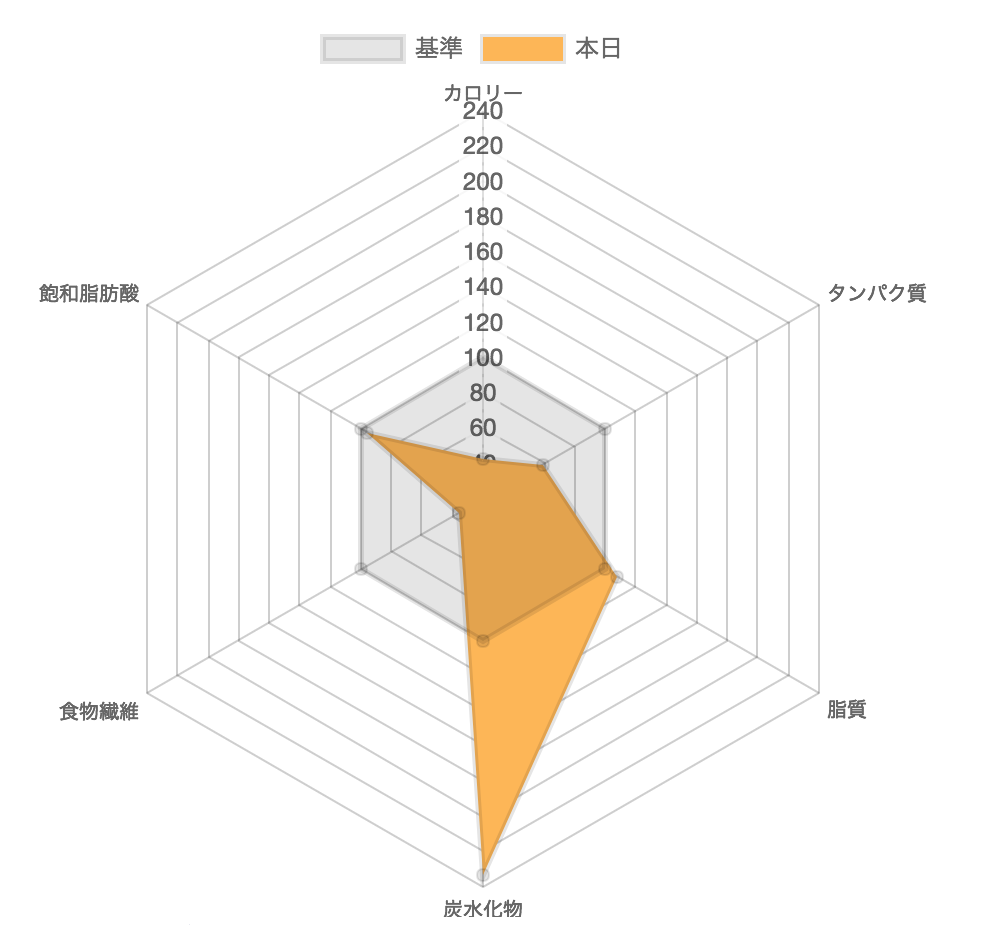
\includegraphics[width=10cm]{imgs/6_radar.png}
        \caption{Webとテレビの画面に表示するレーダーチャート}
        \label{fig:6-radarchart}
    \end{center}
\end{figure}

これにより,ユーザは視覚的に自身の栄養摂取状況が分かる.

フロントエンドでは,見た目を整えるためにBootstrap4を使用した.また一部動的なコンテンツを実装するためにVue.jsを使用した.
テレビ画面の実装には,リアルタイムに撮影された食事画像や家族・医療従事者からのコメントが表示されるようにWebSocketを使用し,Vue.jsを通して表示している.
過去の食事画像やコメントは,RailsのJSON Builderを使用して,フロントエンドからJSONとして受け取れるようにしている.

デプロイ先にはHerokuを使用した.
Herokuを選択した理由は3.2.2で述べた.
アドオンではDBとしてPostgreSQLとRedisを追加し,またメール送信にSendGridを使用した.
フローを設定し,GitHubのリポジトリのdevelopにマージされると自動的にデプロイされるようにした.

また継続的インテグレーションの実現のため,CircleCIを導入した.
CircleCIの設定でrspecを実行するようにして,適宜テストを実行する..
また開発者は全員,gemのpre-commitを使用してコミット前にテストを実行し,テスト失敗時はコミット出来ないようにすることで,不具合を誘発するコードを可能な限り避けるような開発環境を実現した.
\bunseki{佐藤礼於}


\section{料理画像認識の実装}
料理画像の認識には3.2.3で示したように「docomo 画像認識API」を使用している.
このWebAPIは一つの画像につき一つの物体のみの認識に特化しており,複数の食事が写った画像を入力に使用しても全体を一つの料理として捉えて結果を返す.
本システムでは複数の料理を箱に入れても正常に認識が行えることが理想であるため,これを実現するには皿ごとに画像を分け,その皿の枚数だけ「docomo 画像認識API」に入力として与える必要がある.
本グループはOpenCVを使用して二値化閾値処理を行い,皿の範囲を割り出すこととした.
今回のプロダクトでは白い箱を使用するので,背景は常に白であるから,閾値による皿の判別は比較的容易であった.
閾値で皿を識別した後,輪郭を抽出することで皿の判定が可能となった(図\ref{fig:6-threshold}).

\begin{figure}[htbp]
    \begin{center}
        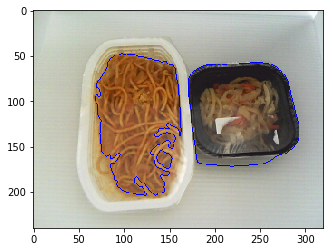
\includegraphics[width=10cm]{imgs/6_threshold.png}
        \caption{閾値によって皿を識別}
        \label{fig:6-threshold}
    \end{center}
\end{figure}

今回は皿ごとの画像に分ける必要があるため,輪郭から外接矩形を検出し,元の画像から皿ごとの画像に切り分けることとした(図\ref{fig:6-bounding}).

\begin{figure}[htbp]
    \begin{center}
        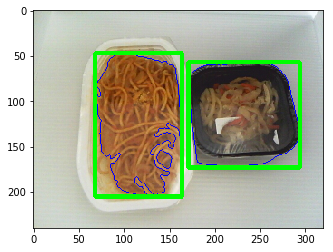
\includegraphics[width=10cm]{imgs/6_bounding.png}
        \caption{外接矩形で皿を囲む}
        \label{fig:6-bounding}
    \end{center}
\end{figure}

皿ごとの画像に切り分けることができたこれらを「docomo 画像認識API」に入力として与えると,複数の候補がJSONで返却される.

本システムでは,最もスコアの高い認識結果をその皿の料理名としてWebサーバに保存するようにしている.
\bunseki{佐藤礼於}

\end{document}
